\chapter{Methodology} \label{chap:methodology}

This chapter will present a multi-level model design flow for the integration of heterogeneous applications and their deployment to the edge on embedded low power devices like NVIDIA Jetson TX2.


\section{A ROS based robotic system}
The choice of the most suitable integration platform is one of the main problems to be faced when integrating heterogeneous applications such as robotic software systems. This choice will have implications on performance and communication of the whole system. Furthermore it will be a key factor during the design phase of the entire architecture.

%TODO da dire meglio non dire "caso specifico" bisogna stare generici.
After an accurate comparison among all available robotics platforms, for the purpose of the specific application developed in this thesis it has been decided to use ROS \cite{ROS} in favour of its standard on communication among other robotic applications.


The design flow proposed in this work is composed of three bottom-up architecture levels, but the same methodology can be applied with more levels.
The purpose of this methodology is to bring an heterogeneous application within an orchestration system such as Kubernetes, and then extend it to the edge computing. % embedded systems
The architecture are explained in the next sections.




\section{First level architecture}
This is the first architecture to start with and the most common used by robotics researches and developers.
At this architecture level the purpose is to verify the functioning of the whole system with the only ROS capabilities on a single powerful machine. A simple scheme of this architecture is shown in figure \ref{fig:l1arch}.

\begin{figure}[htbp]
	\centering
	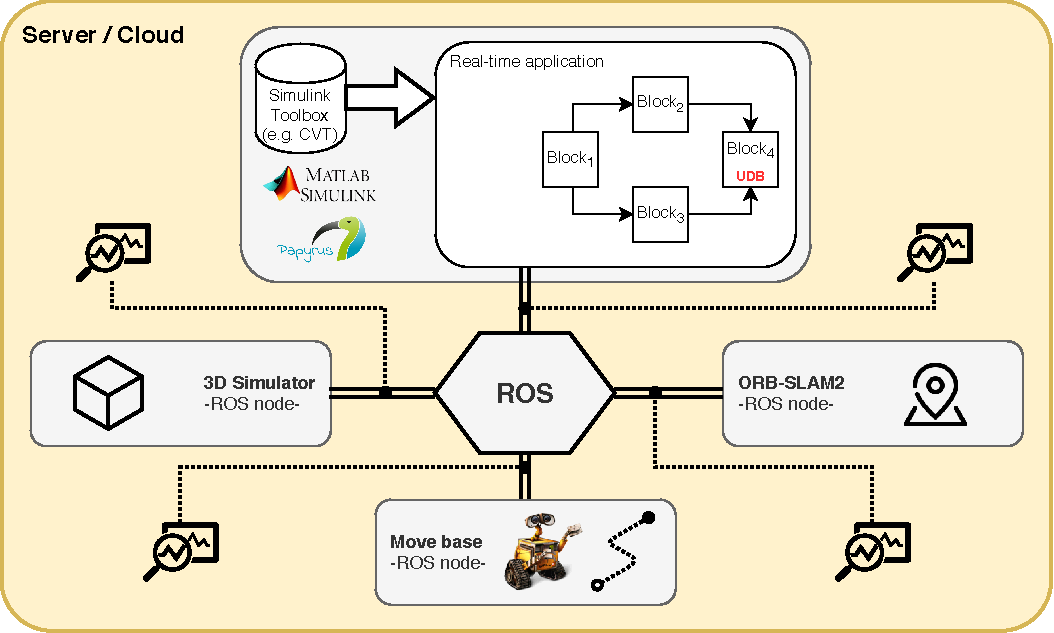
\includegraphics[width=\textwidth]{images/L1-arch}
	\caption{A general architecture at L1}
	\label{fig:l1arch}
\end{figure}

The first step to realize this architecture is to wrap your (heterogeneous) applications with the ROS conformance protocol advertises and callbacks. An example of this operation is provided in listings \ref{lst:pub} and \ref{lst:sub}.
In this way, all the applications that compose your system will be able to interact following the standard communication based on ROS.
The ROS nodes (publishers and subscribers) communicate between them through virtal channels called topics, thus it is necessary choice the right names of these topics and who will read/write on them.
Note that with reference to the  scheme presented in figure \ref{fig:l1arch}, among the other components, there is a robot simulator which have to simulate an industrial robot controller that adheres to the ROS-Industrial driver specification. It means that, for the simulator, we shouldn't choose names and properties of his topics different than the topics published from the robot we are going to develop on. Furthermore all the properties configured in the project withing the simulator should be follow the techniacal specification of the real robot we will use.

Once the applications are ready to run on ROS, they can be executed using a launchfile, where the user can specify a set of nodes to launch and their parameters.
Another possibility is invoke the \mintinline{bash}{rosrun} command for each node that have to be executed.


\noindent\begin{minipage}{.475\textwidth}
\begin{minted}[
frame=single,
framesep=2mm,
baselinestretch=1.2,
fontsize=\footnotesize,
linenos=true,
numbersep=7pt
]{cpp}
#include "ros/ros.h"
...
int main(int argc, char **argv) {
 ros::init(argc, argv, "nodeA");
 ros::NodeHandle n;
 ros::Publisher pub;
 pub=n.advertise<T>("topicT", 10);
 while (ros::ok()) {
  <put here your application>
  ...
  pub.publish(msg);
  ...
 }
 return 0;
}
\end{minted}
\end{minipage}\hfill
\begin{minipage}{.475\textwidth}
\begin{minted}[
frame=single,
framesep=2mm,
baselinestretch=1.2,
fontsize=\footnotesize,
linenos=true,
numbersep=7pt,
breaklines 
]{cpp}
#include "ros/ros.h"
...
void subCallback(const <T> msg) {
 <do stuff with received message>
}

int main(int argc, char **argv) {
 ros::init(argc, argv, "nodeB");
 ros::NodeHandle n;
 ros::Subscriber sub;
 sub=n.subscribe("topicT", 10, subCallback);
 ...
 return 0;
}
\end{minted}
\end{minipage}
\\


Commands such as \mintinline{bash}{rostopic nodes} and \mintinline{bash}{rostopic list} can be used to verify the correct communication between the nodes that compose the system.
There exist more other tools to better inspect an application based on ROS, and they are all available online on ROS documentation.
A good practise for performance measurement in ROS is to use profilers such as: \textit{perf}, \textit{gprof} and \textit{callgrind}. Another profiler tool available in ROS is \mintinline{bash}{rqt_top}, but it doesn't seem very stable and precise yet. Nevertheless, the best choice still put some time points in your code and write the measured intervals on files.



\section{Second level architecture}
Once the system is working properly on a single x86 host machine, it is possible to split it deploying manually the ROS nodes on a low power embedded device.
Again, it is necessary pay attention on communication between nodes, because now they are on different machines and they need to communicate between them through a physical network layer.

It would be preferable to have the control over which ROS nodes run on which machines, for load-balancing and bandwidth management.
Intuitively a user would duplicate the roslaunch files and comment them in a mutually exclusive way, such that the nodes that run on a machine, don't run on the other. Even if it could work correctly, this kind of hard-coding is not the best practice for this purpose, especially for large projects. The recommanded way is to use machine tags to balance load and control which nodes run on the same machine, and consider having the machine file name depend on an environment variable for reusability.

There are some situations, where that's inconvenient or impossible to use the \mintinline{bash}{env} substitution \mintinline{bash}{arg} in order to modifying the behavior without changing any launch files. For example, this is the case when we need for a package that contains a version of the 2d navigation app, but for use in the Gazebo simulator.
For navigation, the only thing that changes is actually that the Gazebo environment is based on a different static map, so the \textit{map\_server} node must be loaded with a different argument. It could be use another \mintinline{bash}{env} substitution here. But that would require the user to set a bunch of environment variables just to be able to roslaunch. 
Instead, it is possible to modify a ``top-level'' aspect of an application, copying the top level launch file and changing the portions you need. 


ROS is designed with distributed computing in mind. A well-written node makes no assumptions about where in the network it runs, allowing computation to be relocated at run-time to match the available resources. Deploying a ROS system across multiple machines require the following:

\begin{itemize}
	\item You only need one master. Select one machine to run it on.
	\item All nodes must be configured to use the same master, setting the ROS\_MASTER\_URI environment variable.
	\item There must be complete, bi-directional connectivity between all pairs of machines, on all ports.
	\item Each machine must advertise itself by a name that all other machines can resolve.
\end{itemize}  

Finally, if the roslaunch files have been properly defined as described above, the only thing to do is copy them as they are on all involved devices, and then run the \mintinline{bash}{roslaunch} command.


%TODO put here an example of general architecture at L2
\begin{figure}[htbp]
	\centering
	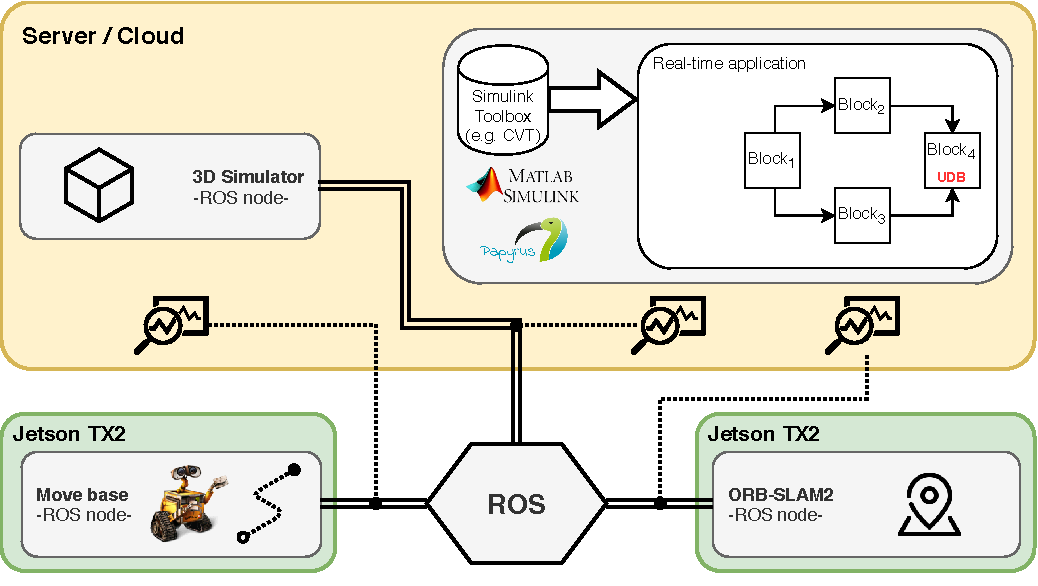
\includegraphics[width=\textwidth]{images/L2-arch}
	\caption{A general architecture at L2}
	\label{fig:l2arch}
\end{figure}


Once again it is very important measure the performance of our system, because we will in the next sections that they will be critical for a correct orchestration of the system.


\section{Third level architecture}
This is the final architecture level. As shown in figure \ref{fig:l3arch} the simulator has been removed and it has been replaced by the real robot.

The difference respect to the previous architecture level is that there there is one or more driver node that communicate with a piece of hardware and it must run on the machine to which the hardware is physically connected.
If the simulator  at L1 has been properly designed and configured, in order to have the system running on the real robot it's enough remove the simulator from the ROS netowrk and attach the robot instead. This operation depend to the physical infrastructure of the netwrok we are on. 

\begin{figure}[htbp]
	\centering
	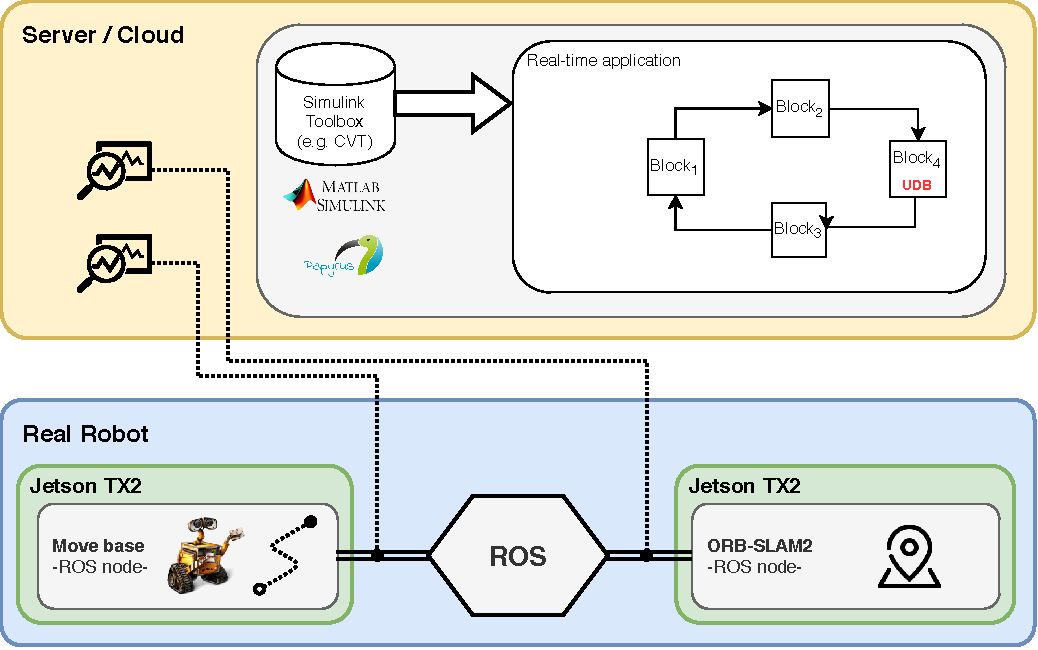
\includegraphics[width=\textwidth]{images/L3-arch}
	\caption{A general architecture at L3}
	\label{fig:l3arch}
\end{figure}


\section{Deploying the system at the edge}
The next step is prepare the system for automatic deployment at the edge. For this purpose we need: first a container platform with which containerize the nodes that compose the system, and then we need for an orchestration platform to automatize the deployment over the cluster of embedded devices.

\subsection{Containerization with Docker}
The use of containers to deploy applications is called containerization. Containers are not new, but their use for easily deploying applications is.
Fundamentally, a container is nothing but a running process, with some added encapsulation features applied to it in order to keep it isolated from the host and from other containers. One of the most important aspects of container isolation is that each container interacts with its own private filesystem; this filesystem is provided by a Docker image. Images include everything needed to run an application - the code or binary, runtimes, dependencies, and any other filesystem objects required.

To develop containerized applications, in general, the development workflow looks like this:
\begin{itemize}
	\item Create and test individual containers for each component of your application by first creating Docker images.
	\item Assemble your containers and supporting infrastructure into a complete application.
	\item Test, share, and deploy your complete containerized application.
\end{itemize}

An image is created only after the definition of a \textit{Dockefile}. Dockerfiles describe how to assemble a private filesystem for a container, and can also contain some metadata describing how to run a container based on this image. An example of Dockerfile looks like this:

\begin{minted}[
frame=single,
framesep=2mm,
baselinestretch=1.2,
fontsize=\footnotesize,
linenos=false,
breaklines 
]{bash}
# Use the official image as a parent image
FROM node:current-slim

# Set the working directory
WORKDIR /usr/src/app

# Copy the file from your host to your current location
COPY package.json .

# Run the command inside your image filesystem
RUN npm install

# Inform Docker that the container is listening on the specified port at runtime.
EXPOSE 8080

# Run the specified command within the container.
CMD [ "npm", "start" ]

# Copy the rest of your app's source code from your host to your image filesystem.
COPY . .
\end{minted}
%\caption{lst:A minimal example of Dockerfile.}


The main server provider of images is Docker Hub \cite{DockerHub} from which it is possible to search for Docker images created for different systems and configurations.
ROS Docker images are listed in the official ROS repository on Docker Hub, therefore this is a good starting point for create an image of a ``simple'' ROS application.
In some cases, when the applications are very heterogeneous and they make use of gpus, a CUDA containerized image (in case of NVIDIA gpus) could be a better starting point.
This is because a CUDA proprietary library could be more tedious to install within the image.

In both cases when we containerize a ROS application, we need to pay attention on two critical points, especially if we a system that must be run on different machines.
The first is that in order to properly source the ROS packages for our application within the container (once it has been created), we must to put the following command at the end of the Dockerfile:

\begin{minted}[breaklines, breakafter=isource]{bash}
RUN . "/opt/ros/$ROS_DISTRO/setup.sh" && sed -i -e '$isource "$CATKIN_WS/devel/setup.bash"' /ros_entrypoint.sh
\end{minted}


Some official ROS images available on the Docker Hub, come already provided of the \textit{ros\_entrypoint} script indicated above. In case it is missing, it is very simple create it in the root of the file system's image. In this way, when a container is starting, before run the \mintinline{bash}{CMD} command, it will source all the necessary ROS packages previously installed within the image.

Before proceeding we need to spend so work about Docker network. Docker’s networking subsystem is pluggable, using drivers. Several drivers exist by default, and provide core networking functionality:
\begin{itemize}
	\item \textbf{User-defined bridge networks} are best when you need multiple containers to communicate on the same Docker host.
	\item \textbf{Host networks} are best when the network stack should not be isolated from the Docker host, but you want other aspects of the container to be isolated.
	\item \textbf{Overlay networks} are best when you need containers running on different Docker hosts to communicate, or when multiple applications work together using swarm services.
	\item \textbf{Macvlan networks} are best when you are migrating from a VM setup or need your containers to look like physical hosts on your network, each with a unique MAC address.
	\item \textbf{Third-party network plugins} allow you to integrate Docker with specialized network stacks.
\end{itemize}
Looking at the above descriptions provided from Docker documentation, when containers will run on different machines it should used the \textit{Overlay networks}. Nevertheless, in case of ROS applications running on multiple host/devices within a container, there is a further problem related to the ports that the ROS system opens. This mean that we can't statically choice what ports open when the container is running, therefore we have to open all of them using the \textit{Host network}.
When we are building the docker image, to enable the communication over the \textit{Host network} we need to run the \mintinline{bash}{build} command with the flag \mintinline{bash}{--network=host}.



Another issue is coming out, when we want to benefit of the hardware resources other than CPU, such as GPUs and tensor cores, provided by the heterogeneous platforms on which we will deploy the applications that compose our system.
Since Docker 19.03, it has been added the support to the NVIDIA-container-runtime. Provided by NVIDIA, it is a modified version of runc adding a custom pre-start hook to all containers.
If environment variable \mintinline{bash}{NVIDIA_VISIBLE_DEVICES} is set in the Open Container Initiative (OCI) specifications, the hook will configure GPU access for the container by leveraging nvidia-container-cli from libnvidia-container project.
There are various methods to setup the docker engine for this purpose. The one proposed by NVIDIA is to register the nvidia runtime reconfiguring the docker daemon configuration file as follow:
\begin{minted}[
frame=single,
framesep=2mm,
fontsize=\footnotesize,
baselinestretch=1.2,
linenos=false,
breaklines
]{json}
{
	"runtimes": {
		"nvidia": {
			"path": "nvidia-container-runtime",
			"runtimeArgs": []
		}
	},
	"default-runtime": "nvidia"
}
\end{minted}

We have already said, that because of a NVIDIA proprietary library could be more tedious to install within a Docker image, the choice to start from an image already provided with gpu (CUDA) libraries would be recommanded. This kind of images are available on the NVIDIA NGC website \cite{nvidiangc}. Once a gpu capable image has been pulled, we can create a container from it simply adding the \mintinline{bash}{--gpus all} flag to the \mintinline{bash}{docker run} or \mintinline{bash}{docker build} commands.

Setting up the Docker platform following the above procedure, will force the system to load some NVIDIA runtime libraries from the host. 
In particular we could have some problem even we are building our (CUDA) application during the build phase of the image, or trying to build them within a running container previously created. 
Most of the available images on the NVIDIA NGC website are missing development versions of the CUDA libraries. A workaround solution for this problem is the manually installation of the these missing libraries ignoring its dependencies. Otherwise the package manager tool will fail the installation.

Moreover, it is important to highlight that the automatic loading of the runtime libraries, performed by the nvidia-container-runtime, involve a strong dependence with the physical device where the these libraries are installed on. Therefore, if we want to deploy the image created in such way, we have to repeat the manually installation of the missing libraries on all devices on which it will be deployed.



\subsection{Deployment}
Finally the system is ready to be distributed on heterogeneous platforms, but it isn't yet ready for an automatic smart deployment and orchestration.
For this purpose we need to do one more thing. First of all, we have to push to the Docker Hub all the images created as described in the previous section. In this way we can pull them from any device wherever they are. Then we need for an orchestration capable platform like Kubernetes (see section \ref{sec:kubernetesbackground}). Moreover with the support of KubeEdge \ref{sec:kubeedgebackground} we can extend the Kubernetes capabilities from the cloud to the edge.

To address all these requirements, we can follow the standard procedure described in KubeEdge documentation \cite{kubeedgedoc}.
KubeEdge is composed of cloud and edge sides. It is built upon Kubernetes and provides core infrastructure support for networking, application deployment and metadata synchronization between cloud and edge. So if we want to setup KubeEdge, we need to setup Kubernetes cluster (existing cluster can be used), cloud side and edge side.
On cloud side, we need to install Docker, Kubernetes cluster and cloudcore. On edge side instead, we need to install Docker, MQTT (We can also use internal MQTT broker) and edgecore. 
After the installation of KubeEdge, setting up cloud side requires two steps: 
\begin{itemize}
	\item Modification of the configuration files.
	\item Edge node manually registration (this is optional because will be auto registered by default).
\end{itemize}

The \textit{cloudconfig.yaml} configuration file can be generated specifying the \mintinline{bash}{--minconfig} argument to the cloudcore binary (see the listing below).
\begin{minted}[
frame=single,
framesep=2mm,
baselinestretch=1.2,
fontsize=\footnotesize,
linenos,
breaklines
]{yaml}
apiVersion: cloudcore.config.kubeedge.io/v1alpha1
kind: CloudCore
kubeAPIConfig:
    kubeConfig: /path/to/.kube/config
    master: ""
modules:
    cloudhub:
        nodeLimit: 10
        tlsCAFile: /etc/kubeedge/ca/rootCA.crt
        tlsCertFile: /etc/kubeedge/certs/edge.crt
        tlsPrivateKeyFile: /etc/kubeedge/certs/edge.key
        unixsocket:
            address: unix:///var/lib/kubeedge/kubeedge.sock
            enable: true
        websocket:
        address: <master node ip-address>
        enable: true
        port: 10000
\end{minted}


This configuration file is suitable for beginners, but a more advances configuration can be generate using \mintinline{bash}{--defaultconfig} flag instead.
The most important lines to pay attention in the listing above, are line 4, where e have to type the right path to the configuration file generating during the kubernetes cluster creation. And line 16 in winch we have to write the (static) ip address of the master node where the cloudcore will run.

To the edge side, the procedure to generate the \textit{edgeconfig.yaml} configuration file is the same of the cloud side: either create a minimal configuration with command \mintinline{bash}{edgecore --minconfig} or a full configuration with command \mintinline{bash}{edgecore --defaultconfig}. It's content is slightly different instead:


\begin{minted}[
frame=single,
framesep=2mm,
baselinestretch=1.2,
fontsize=\footnotesize,
linenos,
breaklines
]{yaml}
apiVersion: edgecore.config.kubeedge.io/v1alpha1
database:
    dataSource: /var/lib/kubeedge/edgecore.db
kind: EdgeCore
modules:
    edged:
        cgroupDriver: cgroupfs
        clusterDNS: ""
        clusterDomain: ""
        devicePluginEnabled: false
        dockerAddress: unix:///var/run/docker.sock
        gpuPluginEnabled: true
        hostnameOverride: <edge node name>
        interfaceName: eth0
        nodeIP: <edge node ip-address>
        podSandboxImage: kubeedge/pause-arm64:3.1
        remoteImageEndpoint: unix:///var/run/dockershim.sock
        remoteRuntimeEndpoint: unix:///var/run/dockershim.sock
        runtimeType: docker
    edgehub:
        heartbeat: 15
        tlsCaFile: /etc/kubeedge/ca/rootCA.crt
        tlsCertFile: /etc/kubeedge/certs/edge.crt
        tlsPrivateKeyFile: /etc/kubeedge/certs/edge.key
        websocket:
            enable: true
            handshakeTimeout: 30
            readDeadline: 15
            server: <master node ip-address>:10000
            writeDeadline: 15
    eventbus:
        mqttMode: 2
        mqttQOS: 0
        mqttRetain: false
        mqttServerExternal: tcp://127.0.0.1:1883
        mqttServerInternal: tcp://127.0.0.1:1884
\end{minted}


In this case the lines to pay attention are line 13, where we have to write the node name (necessary for deployments). Line 15 where we have to type (static) ip address of the edge node. Finally the line is the ip and port where the server socket of the master node is listening on, and it must to be the same of line 16 in the \textit{cloudconfig.yaml}.

Now, that the cluster is set up, we are ready to write the last three configuration files necessary for the device controller in order to automatically deploy our containerized applications to the edge nodes.
The device controller is the cloud component of KubeEdge which is responsible for device management. Device management in KubeEdge is implemented by making use of Kubernetes Custom Resource Definitions (CRDs) to describe device metadata/status and device controller to synchronize these device updates between edge and cloud. The device controller starts two separate go-routines called \textit{upstream controller} and \textit{downstream controller}. These are not separate controllers as such but named here for clarity.
The device controller makes use of device model and device instance to implement device management :
A device model describes the device properties exposed by the device and property visitors to access these properties. A device model is like a reusable template using which many devices can be created and managed. A device instance represents an actual device object. It is like an instantiation of the device model and references properties defined in the model. The device spec is static while the device status contains dynamically changing data like the desired state of a device property and the state reported by the device.
Generally the steps to address these requirements are the following:
\begin{enumerate}
	\item Create a device model in the cloud node.
	\item Create a device instance in the cloud node.
	\item Run the mapper application corresponding to your protocol.
	\item Edit the status section of the device instance yaml created in step 2 and apply the yaml to change the state of device twin. This change will be reflected at the edge, through the device controller and device twin modules. Based on the updated value of device twin at the edge the mapper will be able to perform its operation on the device.
	\item The reported values of the device twin are updated by the mapper application at the edge and this data is synced back to the cloud by the device controller. User can view the update at the cloud by checking his device instance object.
\end{enumerate}

Note: Creation of device instance will also lead to the creation of a config map which will contain information about the devices which are required by the mapper applications The name of the config map will be as follows: device-profile-config-< edge node name >. The updation of the config map is handled internally by the device controller.
Further details on both device model and device instance definition can be found on Kubeedge documentation.

An example of device model, device instance and deployment configuration files are shown below:

\inputminted[frame=single,
framesep=2mm,
baselinestretch=1.2,
fontsize=\footnotesize,
linenos,
breaklines]{yaml}{sourcecode/led-light-device-model.yaml}


\inputminted[frame=single,
framesep=2mm,
baselinestretch=1.2,
fontsize=\footnotesize,
linenos,
breaklines]{yaml}{sourcecode/led-light-device-instance.yaml}


\inputminted[frame=single,
framesep=2mm,
baselinestretch=1.2,
fontsize=\footnotesize,
linenos,
breaklines]{yaml}{sourcecode/deployment.yaml}


Finally we can create/apply these configuration files files using the kubectl commands and leave KubeEdge the creation, distribution and management of the pods related to the our applications.

% qui volendo possiamo parlare di misurazione delle performane e memory footprint.
% http://docs.kubeedge.io/en/latest/setup/memfootprint-test-setup.html



\clearpage
\thispagestyle{empty}



















